\documentclass{article}

\usepackage{polski}
\usepackage{amsmath}
\usepackage{graphicx}
\usepackage{float}
\usepackage{subfig}
\usepackage{multirow}

\title{Aproksymacja średniokwadratowa wielomianami trygonometrycznymi}
\author{\textbf{Łukasz Wala}\\
    \textit{AGH, Wydział Informatyki, Elektroniki i Telekomunikacji} \\
    \textit{Metody Obliczeniowe w Nauce i Technice 2021/2022}}
\date{Kraków, \today}

\begin{document}
\maketitle

\section{Opis problemu}
Główną ideą zadania jest zbadanie zachowania funkcji przybliżonej za pomocą aproksymacji
średniokwadratowej wielomianami trygonometrycznymi.

Badana funkcja:
\[f(x)=x^2-m\cdot\cos\left(\frac{\pi x}{k}\right)\]
Gdzie $k=\frac{1}{2}$, $m=4$ oraz $x\in [-6,6]$.

\section{Opracowanie}
\subsection{Wyprowadzenie}
W aproksymacji średniokwadratowej poszukiwana jest wartość minimalna sumy kwadratów różnic funkcji aproksymowanej $F(x)$
oraz funkcji aproksymującej $f(x)$ z uwzględnieniem funkcji wagowej $w(x)$ większej od zera (tutaj $\forall x \in D
:w(x) = 1$). Funkcją aproksymującą ma być wielomian trygonometrycznym o postaci
$$\displaystyle f(x) = a_0 + \sum_{j=1}^mb_j\cos(jx)\:+\:\sum_{j=1}^m a_j\sin(jx)$$

Więc błąd średniokwadratowy przyjmuje postać

$$\displaystyle H(a_0, ..., a_m, b_1, ..., b_m)=\sum_{i=1}^nw(x_i)\left[F(x_i)-(a_0 + \sum_{j=1}^mb_j\cos(jx_i)\:+\:\sum_{j=1}^m a_j\sin(jx_i))\right]^2$$

Aby funkcja przyjmowała wartość minimalną względem współczynnka $c$, pochodna funkcji względem tego współczynnika musi
wynosić zero

$$\frac{\partial H}{\partial c}=0, c \in \{a_0, ..., a_m, b_1, ..., b_m\}$$

Na przykład dla $a_k$

$$\displaystyle -2\sum_{i=1}^nw(x_i)\left[F(x_i)-(a_0 + \sum_{j=1}^mb_j\sin(jx_i)\:+\:\sum_{j=1}^m a_j\cos(jx_i))\right]\cos(kx_i) = 0$$

Po przekształceniach dla $a_0$
\begin{multline*}
    $$\displaystyle \sum_{i=0}^nw(x_i)a_0+\sum_{j=1}^m\left(\sum_{i=0}^nw(x_i)\cos(jx_i)\right)a_j+
    \sum_{j=1}^m\left(\sum_{i=0}^nw(x_i)\sin(jx_i)\right)b_j \\=\sum_{i=0}^nw(x_i)F(x_i)$$
\end{multline*}

Dla $a_k, k\in\{1,2,...,m\}$:
\begin{multline*}
    $$\displaystyle \sum_{i=0}^nw(x_i)\cos(kx_i)a_0+\sum_{j=1}^m\left(\sum_{i=0}^nw(x_i)\cos(kx_i)\cos(jx_i)\right)a_j+
    \sum_{j=1}^m\left(\sum_{i=0}^nw(x_i)\cos(kx_i)\sin(jx_i)\right)b_j \\ =\sum_{i=0}^nw(x_i)F(x_i)\cos(kx_i)$$
\end{multline*}

Oraz dla $b_k, k\in\{1,2,...,m\}$
\begin{multline*}
    $$\displaystyle \sum_{i=0}^nw(x_i)\sin(kx_i)a_0+\sum_{j=1}^m\left(\sum_{i=0}^nw(x_i)\sin(kx_i)\cos(jx_i)\right)a_j+
    \sum_{j=1}^m\left(\sum_{i=0}^nw(x_i)\sin(kx_i)\sin(jx_i)\right)b_j \\ =\sum_{i=0}^nw(x_i)F(x_i)\sin(kx_i)$$
\end{multline*}

Z tych równań można zbudować układ
\[
\begin{bmatrix}
    \sum_{i=0}^nw(x_i) & \sum_{i=0}^nw(x_i)\cos(1\cdot x_i) & \sum_{i=0}^nw(x_i)\sin(1\cdot x_i) & \hdots \\
    \sum_{i=0}^nw(x_i)\cos(1\cdot x_i) & \sum_{i=0}^nw(x_i)\cos(1\cdot x_i)\cos(1\cdot x_i) & \sum_{i=0}^nw(x_i)\cos(1\cdot x_i)\sin(1\cdot x_i) & \hdots\\
    \sum_{i=0}^nw(x_i)\sin(1\cdot x_i) & \sum_{i=0}^nw(x_i)\sin(1\cdot x_i)\cos(1\cdot x_i) & \sum_{i=0}^nw(x_i)\sin(1\cdot x_i)\sin(1\cdot x_i) & \hdots\\
    \sum_{i=0}^nw(x_i)\cos(2\cdot x_i) & \sum_{i=0}^nw(x_i)\cos(2\cdot x_i)\cos(1\cdot x_i) & \sum_{i=0}^nw(x_i)\cos(2\cdot x_i)\sin(1\cdot x_i) & \hdots\\
    \sum_{i=0}^nw(x_i)\sin(2\cdot x_i) & \sum_{i=0}^nw(x_i)\sin(2\cdot x_i)\cos(1\cdot x_i) & \sum_{i=0}^nw(x_i)\sin(2\cdot x_i)\sin(1\cdot x_i) & \hdots\\
    \vdots & \vdots & \vdots & \vdots \\
    \sum_{i=0}^nw(x_i)\cos(m\cdot x_i) & \sum_{i=0}^nw(x_i)\cos(m\cdot x_i)\cos(1\cdot x_i) & \sum_{i=0}^nw(x_i)\cos(m\cdot x_i)\sin(1\cdot x_i) & \hdots\\
    \sum_{i=0}^nw(x_i)\sin(m\cdot x_i) & \sum_{i=0}^nw(x_i)\sin(m\cdot x_i)\cos(1\cdot x_i) & \sum_{i=0}^nw(x_i)\sin(m\cdot x_i)\sin(1\cdot x_i) & \hdots\\
\end{bmatrix}
\cdot
\]

\[
\cdot
\begin{bmatrix}
    a_0 \\
    a_1 \\
    b_1 \\
    a_2 \\
    b_2 \\
    \vdots \\
    a_m \\
    b_m \\ 
\end{bmatrix}
=
\begin{bmatrix}
    \sum_{i=0}^nw(x_i)F(x_i) \\
    \sum_{i=0}^nw(x_i)F(x_i)\cos(1\cdot x_i) \\
    \sum_{i=0}^nw(x_i)F(x_i)\sin(1\cdot x_i) \\
    \sum_{i=0}^nw(x_i)F(x_i)\cos(2\cdot x_i) \\
    \sum_{i=0}^nw(x_i)F(x_i)\sin(2\cdot x_i) \\
    \vdots \\
    \sum_{i=0}^nw(x_i)F(x_i)\cos(m\cdot x_i) \\ 
    \sum_{i=0}^nw(x_i)F(x_i)\sin(m\cdot x_i)
\end{bmatrix}    
\]

Do rozwiązania powyższego układu równań użyta została funkcja \textit{linalg.solve} z pakietu \textit{numpy}
w języku Python.

\subsection{Wykresy}
Pierwszym krokiem analizy będzie zbadanie zachowania wykresów funkcji aproksymujących. Zakres liczby punktów użytych do
stworzenia funkcj wynosi 7-50 z wykorzystaniem wielomianów stopni 3-30 (2 * stopień + 1 = liczba funkcji bazowych), przy 
zachowaniu założenia, że stopień wielomianu musi być większy lub równy liczbie funkcji bazowych. Punkty rozłożone są
równomierne na przedziale.

\begin{figure}[H]
    \centering
    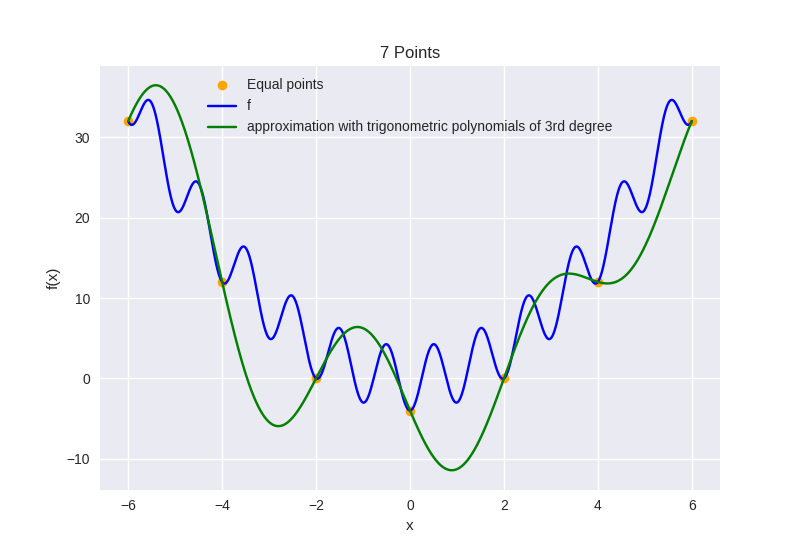
\includegraphics[width=\textwidth]{img/tripoly_3_7.png}
    \caption{Aproksymacja średniokwadratowa wielomianami trygonometrycznymi 3 stopnia}
\end{figure}

\begin{figure}[H]
    \centering
    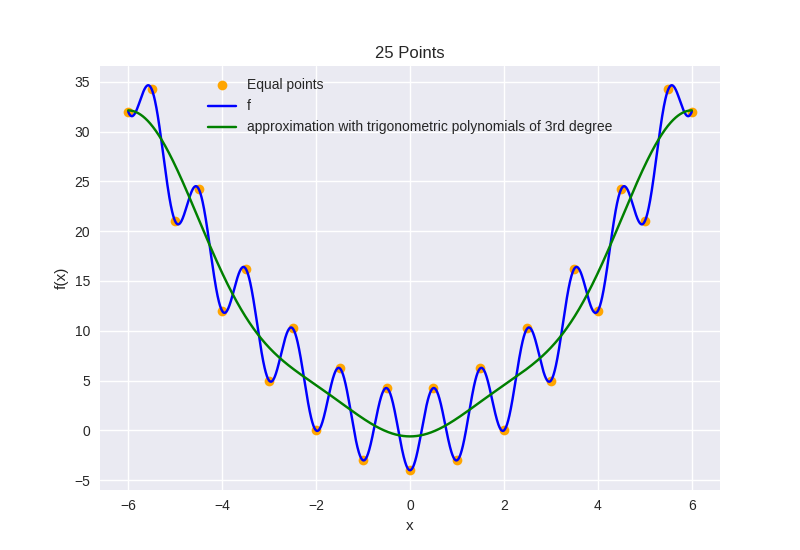
\includegraphics[width=\textwidth]{img/tripoly_3_25.png}
    \caption{Aproksymacja średniokwadratowa wielomianami trygonometrycznymi 3 stopnia}
\end{figure}

Wielomiany trzeciego stopnia (czyli o 7 funkcjach bazowych) nie są na tyle dokładne, żeby odtworzyć w satysfakcjonujący
sposób funkcję aproksymowaną. Zwiększanie liczby punktów pozytywnie wpływa na kształt funkcji, jednak tylko do pewnej wartości
(ok. 17), po której dokładność prawie nie wzrasta.

\begin{figure}[H]
    \centering
    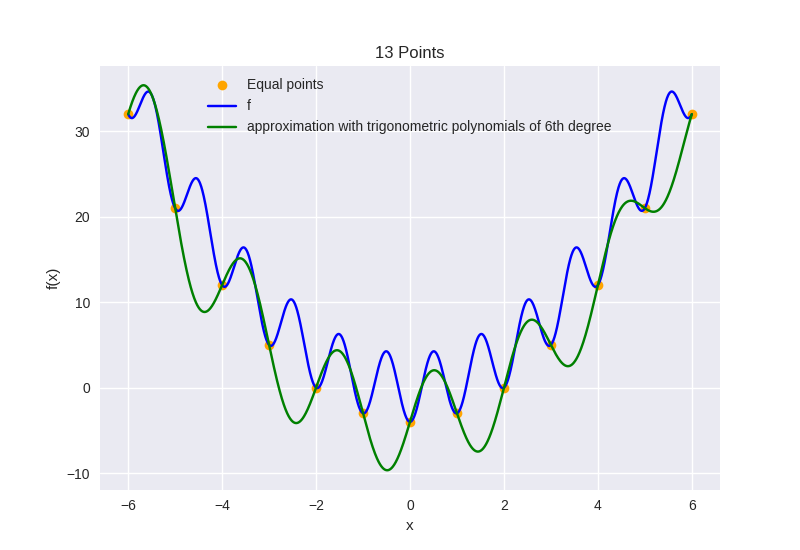
\includegraphics[width=0.9\textwidth]{img/tripoly_6_13.png}
    \caption{Aproksymacja średniokwadratowa wielomianami trygonometrycznymi 6 stopnia}
\end{figure}

\begin{figure}[H]
    \centering
    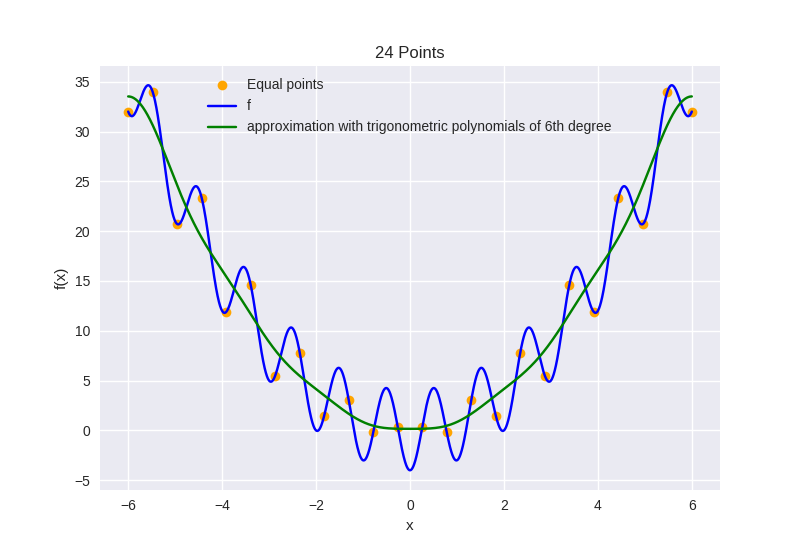
\includegraphics[width=0.9\textwidth]{img/tripoly_6_24.png}
    \caption{Aproksymacja średniokwadratowa wielomianami trygonometrycznymi 6 stopnia}
\end{figure}

Wielomiany szóstego stopnia dla mniejszych liczb węzłów bardziej przypominają wykres funkcji aproksymowanej, zawierają kilka
charakterystycznych "zębów", jednak ze wzrostem liczby punktów, wykres się wygładza, ponieważ stopień jest zbyt niski, żeby
wiernie odwzorować funkcję $f$.

Wielomiany wyższych stopni wykazują podobną tendencję: dla niewielkich liczb węzłów mają więcej głębokich minimów i wysokich maksimów,
częściowo pokazują charakterystyczny kształt funkcji $f$, jednak gdy liczba punktów względem stopnia wielomianu staje się zbyt duża,
wygładzają się, tak więc liczba węzłów nie poprawia drastycznie dokładności.

\begin{figure}[H]
    \centering
    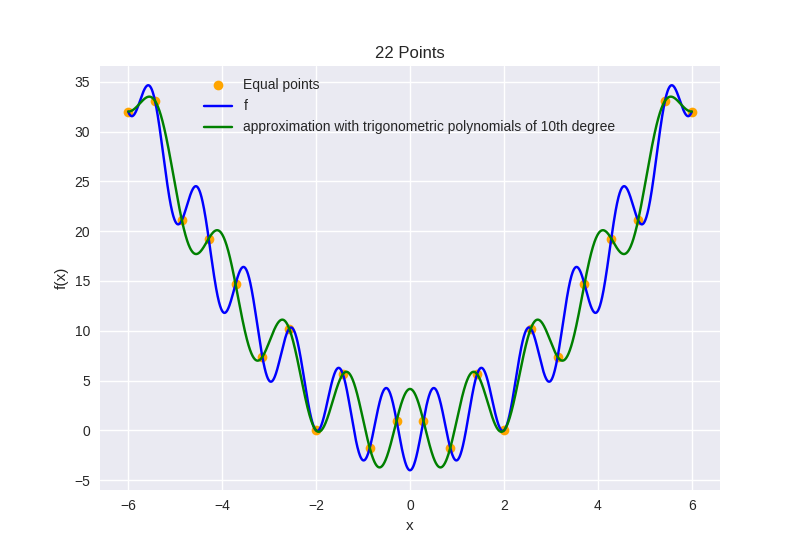
\includegraphics[width=\textwidth]{img/tripoly_10_22.png}
    \caption{Aproksymacja średniokwadratowa wielomianami trygonometrycznymi 10 stopnia}
\end{figure}

\begin{figure}[H]
    \centering
    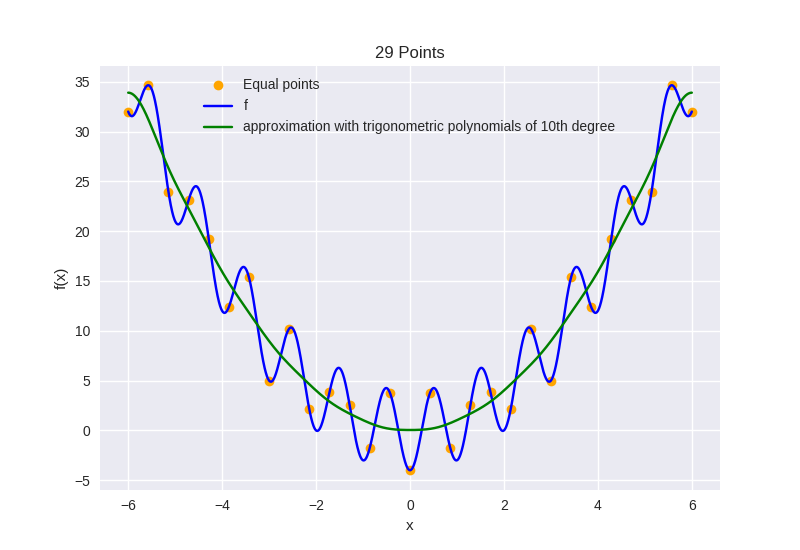
\includegraphics[width=\textwidth]{img/tripoly_10_29.png}
    \caption{Aproksymacja średniokwadratowa wielomianami trygonometrycznymi 10 stopnia}
\end{figure}

Najmniejszy stopień wielomianu, przy którym kształt funkcji jest dobrze odwzorowany, to dwanaście. Przy tej liczbie, dla najmniejszej poprawnej liczby
węzłów, wykresy funkcji aproksymowanej i aproksymacyjnej pokrywają się w bardzo dużym stopniu, zwiększanie liczby węzłów nie daje natomiast
dużej poprawy.

\begin{figure}[H]
    \centering
    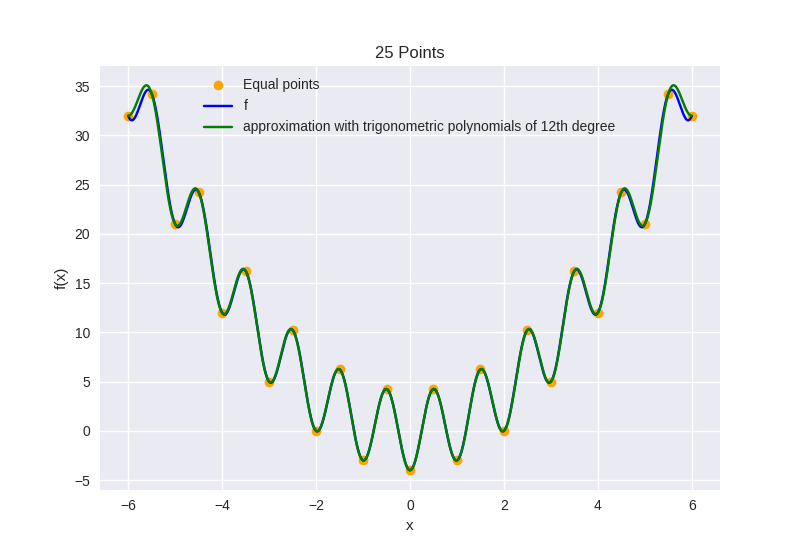
\includegraphics[width=0.9\textwidth]{img/tripoly_12_25.png}
    \caption{Aproksymacja średniokwadratowa wielomianami trygonometrycznymi 12 stopnia}
\end{figure}

\begin{figure}[H]
    \centering
    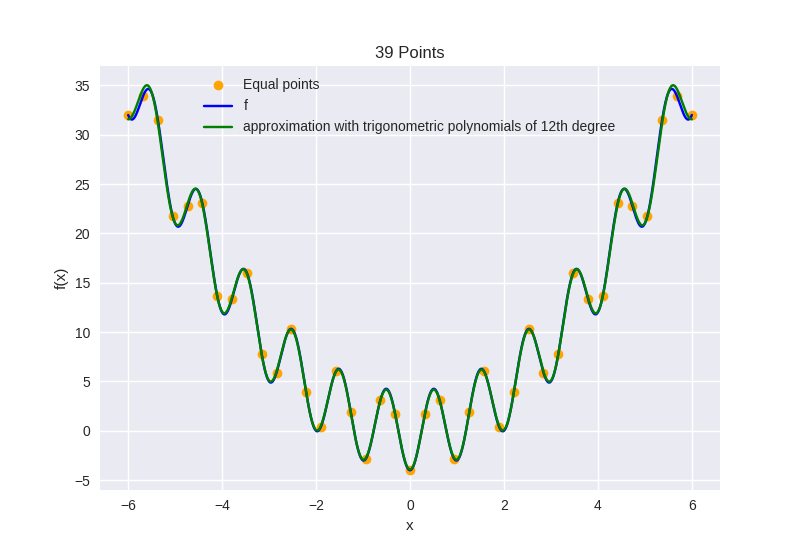
\includegraphics[width=0.9\textwidth]{img/tripoly_12_39.png}
    \caption{Aproksymacja średniokwadratowa wielomianami trygonometrycznymi 12 stopnia}
\end{figure}

Jak widać, zwiększanie liczby węzłów nie już zwiększa zbytnio dokładności. Poniżej wykres dla dwudziestego stopnia wielomianu,
jego dokładność nie zwiększyła się zbytnio w porównaniu do dwunastego stopnia (który był już bardzo dokładny).

\begin{figure}[H]
    \centering
    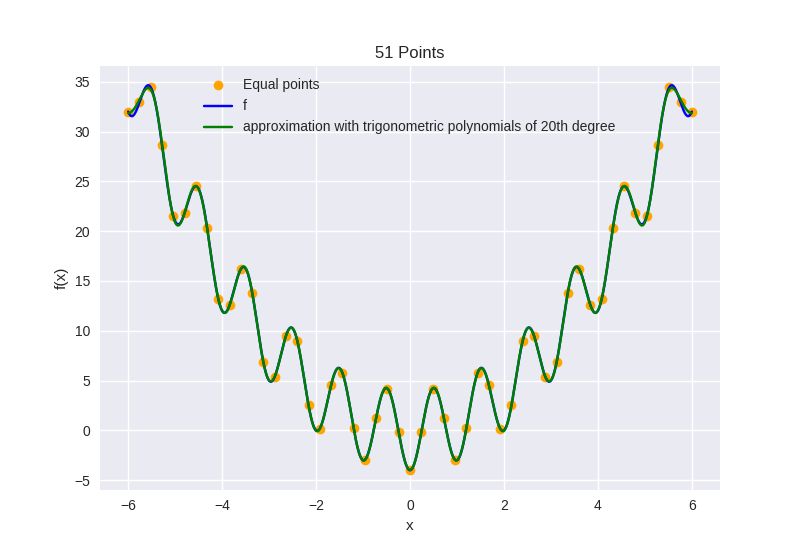
\includegraphics[width=\textwidth]{img/tripoly_20_51.png}
    \caption{Aproksymacja średniokwadratowa wielomianami trygonometrycznymi 20 stopnia}
\end{figure}

\subsection{Dokładności}
Pozostaje obliczenie dokładności oraz skonfrontowanie wyników z wnioskami uzyskanymi na podstawie analizy wykresów. Miarami dokładności będą:
\begin{itemize}
    \item
    średnia kwadratów odległości wartości wielomianu oraz funkcji $f$ dla 1000 równo oddalonych punktów,
    \item
    maksymalna odległość wartości wielomianu oraz funkcji $f$ dla 1000 równo oddalonych punktów.
\end{itemize}


\section{Wnioski}


\end{document}